\section{implementation}

\label{sec:implementation}

\begin{figure} \centering
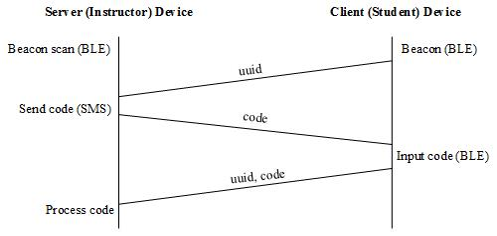
\includegraphics[width=\columnwidth]{figures/bleats-design.png}
\caption{Bleats authentication system design}
\label{fig:bleats-design} \end{figure}

The current BLEATS system consists of two main components. The functional
BLEATS system and the BLEATS simulation. This section will describe in detail
the implementation of each of these components of the BLEATS project.

\subsection{Functional system}

The current BLEATS system is implemented for both the client (student) device
and the server (instructor) device. The student device in the current BLEATS
system is modeled by a Raspberry Pi 2 with a piBeacon from Adafruit~\cite{adafruit}
providing BLE support. The instructor device in the current BLEATS system is
implemented on an Ubuntu 14.04 LTS virtual machine that is dedicated 4 GB RAM,
a 20 GB hard drive, and 2 processors. The code for the BLEATS implementation is
written in the Python programming language. This section will describe first
the student device implementation, then the instructor device implementation,
and will finish with a description of the interaction between the two.

\subsubsection{Student Device}

The student device for the BLEATS system requires two interaction points. The
first interaction point is in the initiation of a BLE beacon to check in with
the instructor for the first form of authentication. This beacon is sent using
a Python library called PyBluez~\cite{pybluez}. PyBluez is a library for Python
that allows interaction with Bluetooth resources on the host machine. The first
BLE beacon is sent from the student device with a unique UUID that is specific
to that student. The major and minor values of the BLE beacon protocol are set
to “1” for this initial beacon.

The second interaction point is the student mobile device receiving the one
time code through SMS from the instructor and sending the code back to the
instructor. The device used to receive the code in the current BLEATS
implementation is a Samsung Galaxy Note 5. Once the code is received, a program
is needed to send the one time code back to the instructor through BLE beacon.
This program again uses the PyBluez to form another BLE beacon message. This
second beacon message again uses the student’s unique UUID for the UUID in the
beacon message. However, for this beacon message, the major value in the beacon
message is set to “5” and the minor value in the beacon message is set to the
one time code that the student received. 

\subsubsection{Instructor Device}

The instructor device for the BLEATS system requires only one interaction point
and runs automatically after initiation. The instructor program uses the
PyBluez library described previously for BLE support. The instructor program
uses SQLite Version 3~\cite{sqlite} for database interaction and
SMTPLib~\cite{smtplib} for transmission of SMS communication. 

The instructor program begins by scanning for BLE packets. After finishing this
scan, the instructor program iterates through each packet it extracted. If the
major value in the packet is equal to 1, then it searches a student database
for a student that has the UUID specified in the packet. After this, the
instructor program creates a one time code by generating a random code between
11111 and 65535. The reasoning behind this range is that 65535 is the upper
limit for the minor value in a BLE beacon packet. After the code is generated,
the instructor program updates an authentication database’s entry for that
student’s UUID with the generated code as well as the current time. The
instructor program also updates an “attempts” counter in the authentication
database at this time as well. Following this, the instructor program sends an
SMS message from a BLEATS Gmail address to the student’s mobile phone. In the
current implementation of the BLEATS system, this is a static implementation
for one student with a static phone number. In a full BLEATS implementation, a
database would be created containing the students’ phone numbers. 

If the major value from a BLE beacon is equal to 5, then the instructor program
processes the packet as the second form of authentication from a student. As
such, the instructor program first ensures that there is a student in the
authentication database with the beacon’s UUID and the one time code that was
sent in the minor value of the beacon packet. If this check passes, the
instructor program checks the current time compared to the time that is in the
student’s authentication database entry and checks the number of attempts that
the code has been sent for that student. If the difference in time is greater
than 60 seconds and the attempts is less than 3, then the instructor program
generates a new one time code and repeats the code sending process detailed
previously. If the difference in time is greater than 60 seconds and the
attempts is 3 or more, then the instructor program will determine that the
student is not present in the classroom. If the difference in time is less than
60 seconds then the instructor program sets the attempt number for the student
to zero attempts and determines that the student is present in the classroom. 

\subsubsection{Student and Instructor Device Interaction}

The interaction between the student and instructor devices is summarized by
Figure~\ref{fig:bleats-design} . First the instructor and student devices begin
scanning for BLE beacons and sending a BLE beacon respectively. The UUID for
the student is transmitted in the student device’s BLE beacon and this is
received by the instructor device. At this time, the instructor device sends a
one time code to the student’s device through SMS messaging. When the student
device receives a code, the student enters this code to their device and the
device transmits another BLE beacon with the student’s UUID and the one time
code. When the instructor device sees this BLE packet, it processes the code
and determines if it should determine the student is present, not present, or
if it should send a new one time code to the student.

\subsection{Simulation}

We used the ns3 network simulator to emulate the performance characteristics of
the BLEATS platform. There is currently no Bluetooth Low Energy module
available for ns3, so we had to construct our own. We modified the 802.15.4
low-rate WPAN~\cite{802-15-4-spec} base module to create a realistic passive
BLE beacon module~\cite{ble-spec}, performing the following tasks: 

\begin{itemize}

\item \textit{Removing CSMA/CA} - BLE passive-mode beaconing uses short
messages and does not does not do carrier sensing to reduce energy consumption. 

\item \textit{Removing all message acknowledgments} - Acknowledging broadcast
messages can be overwhelming in high-density environments, and without
acknowledgments, transmitting beacons can broadcast and then sleep immediately
to reduce energy consumption. Typically acknowledgments are a mechanism for
guaranteeing message delivery, but we instead rely on statistical guarantees
that the message will be delivered over time.

\item \textit{Removing direct address messaging} - There is not point-to-point
communication for passive-mode BLE, and all messages are sent to a broadcast
address and received by all listening nodes. 

\item \textit{Changing parameters} - Many BLE specific parameters and constants
needed to be set; for example, max packet size (47 bytes), data transmission
rate (1 Mbps), transmission duration (\SI{625}{\micro\second}), and maximum
transmission power (10 dBm). 

\item \textit{Remove adaptive physical layer transmission} - BLE operates on a
single frequency hop spread spectrum (FHSS) / Gaussian frequency-shift keying
GFSK physical layer, rather than using the adaptive 802.15.4 physical layer
specification.

\item \textit{Spectrum division} - BLE divides the 2.4-2.4835 GHz band into 40
2-MHz channels rather than 83 1-MHz channels.

\item \textit{Adding random jitter} - BLE adds up to 10ms transmission delay
for collision avoidance with other beacons on the same initial interval offset.

\end{itemize}

There are also a few notable aspects of the LR-WPAN module that we did not
modify from the original 802.15.4 specification:

\begin{itemize}

\item \textit{Physical layer binomial bit error rate (BER) model} - The default
physical error model is meant for offset quadrature phase-shift keying (OQPSK),
binary phase-shift keying (BPSK), or amplitude-shift keying (ASK). This was not
modified because it is a generic additive white Gaussian noise model across the
same bandwidth. While the specific parameters vary in reality, the same general
BER trends apply for BLE’s GFSK physical layer. 

\item \textit{Single channel broadcast} - The BLE specification requires
advertising beacon packets to  be consecutively transmitted across the three
advertising channels (37, 38, 39), but receiver behavior varies by
implementation across vendors that is often closed source. Thus, we did not
attempt to model multiple advertising channels with different receiver
behaviors, and performed simulations on a single broadcast channel. The
observations from single channel advertisement beacons translate easily to a
multiple channel context. 

\end{itemize}
